\documentclass[]{report}
\usepackage{graphicx}
\usepackage{array}
\usepackage[margin=1.0in]{geometry}
% Title Page
\title{User's Guide for the Modular Injection System and Sampling Template (M.I.S.S.T)}  
\author{Froylan Aguirre\\class of '18}


\begin{document}
\maketitle

\chapter*{Foreword}
The purpose of this guide is to aid future MISST developers and users. This guide will:
\begin{itemize}
	\item Give a brief overview of MISST system capabilities.
	\item Provide development advice.
	\item Outline the project's current state.
\end{itemize}

I wrote this guide based on my experience and I hope future developers continue to do so. 

%---------------------------------------------------------------------
\part{The MISST System}

\chapter{Terminology and High Level Concepts}

\section{Introduction}
\label {introduction}
In this chapter, we will describe MISST system high level behavior. For more details, refer to the Design Guide.

\section{System Capabilities and Overall Function}
\label{system capabilities}
The fault injection system was designed as a System on Chip fault injector module that can be added to a prototype for fault tolerance testing. For example, a researcher could observe the behavior of a bus-based micro-processor system prototype after injecting faults into the prototype's peripherals or CPU. 
The following list outlines the steps of using MISST:
\begin{enumerate}
	\item Read documentation and download source code.
	\item Implement Adapter module for specific case.
	\item Test Adapter module compatibility with MISST and target DUT.
	\item Once confirmed to function, program FPGA with test setup.
	\item Configure MISST registers for desired testing parameters. Refer to Design Guide for register details.
	\item Start fault injection campaign, and wait for its end.
	\item Collect and analyze data.
\end{enumerate}

The fault injection system injects faults into a device under test (DUT) and samples specified addresses in that DUT's address space. It is important to note that the DUT and fault injection system are implemented on the same die or programmable logic fabric. How the DUT and fault injection system interface is left to the researcher, and their responsibility to implement a module that allows communication of the fault injection system with the DUT and a PC. See chapter \ref{c adapter setup} for adapter setup details.
After the Adapter is completed, the user must configure the fault injection system by setting system registers to appropriate values. These registers control what, how , and when faults are injected and samples are taken. See \textbf{Memory Organization} section of Design Guide for more details. Then the fault injection is prompted to start injecting faults. The system samples data from the DUT and sends it to a PC when sampling time has been reached. In between sampling events, MISST injects faults into the DUT. This is repeated until a stop condition is reached.
In the next section we will introduce important concepts.

\section{Concepts and Terminology}
\label{concepts and terminology}

A fault can be identified by three characteristics shown in Table \ref{table:fault chars}. Between DUT resets, a specified number of faults are injected, and this grouping is called a \textit{set}. After every set, the fault injection system always samples data from the DUT. See Figure \ref{fig:casecharacteristics} for a visual of an injected fault.

\begin{table}[h]
	\centering
	\caption{Fault Characteristics}
	\begin{tabular}{|c|l|}
		\hline
		Characteristic & Description \\ 
		\hline
		Location & Address of fault location in DUT address space. \\ 
		\hline 
		Time & Time after previous fault or system start (if first fault in a set) measured in DUT clock cycles. \\ 
		\hline 
		Type & How data is corrupted. Examples: bit flip, additive error, etc \\ 
		\hline 
	\end{tabular} 
	\label{table:fault chars}
\end{table}

\begin{figure}[h]
	\centering
	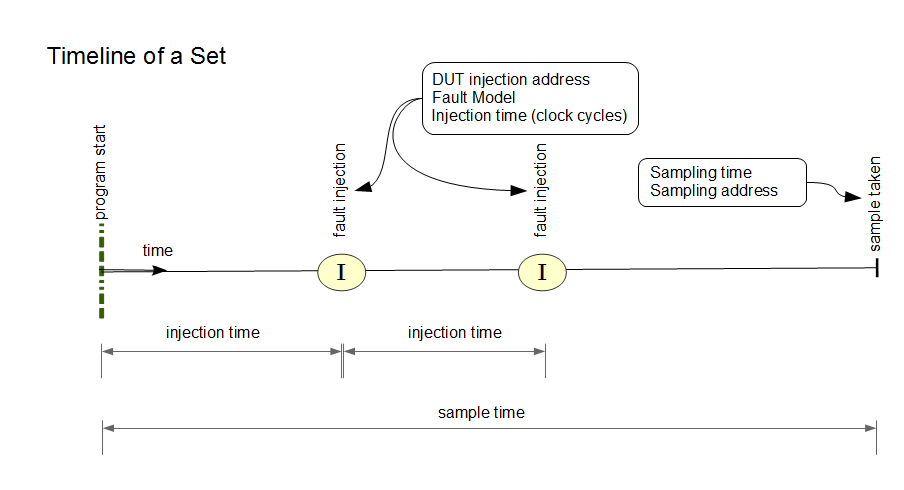
\includegraphics[width=1.0\linewidth]{../technical_diags/f22_timeline_of_set.png}
	\caption{Case characteristics.}
	\label{fig:casecharacteristics}
\end{figure}

The fault injection system will normally repeat a cycle of DUT reset, injecting a set of faults, and sampling until a stop condition is reached. We will refer to this cycle as an campaign throughout this document.

\subsection{Fault Generation}
If sets contain multiple faults, and there are multiple sets within a campaign, how are these faults generated? Do faults change between sets or within sets? This section will explain how fault characteristics change between system resets and between injections within sets. The user should keep the following settings in mind when designing a fault injection campaign:
\begin{itemize}
	\item Initial fault parameter values.
	\item Number of faults in sets.
	\item How fault parameters change.
\end{itemize}

Figure \ref{fig:two_ways_sets} shows two ways faults can change within and without sets. In case 1, the same fault is injected multiple times within a set. In case 2, faults change inside sets. 
For example, case 2 could show that within sets, the location of the fault changes, but between the sets, another fault characteristic (like timing or fault type) changes.

\begin{figure}[h]
	\centering
	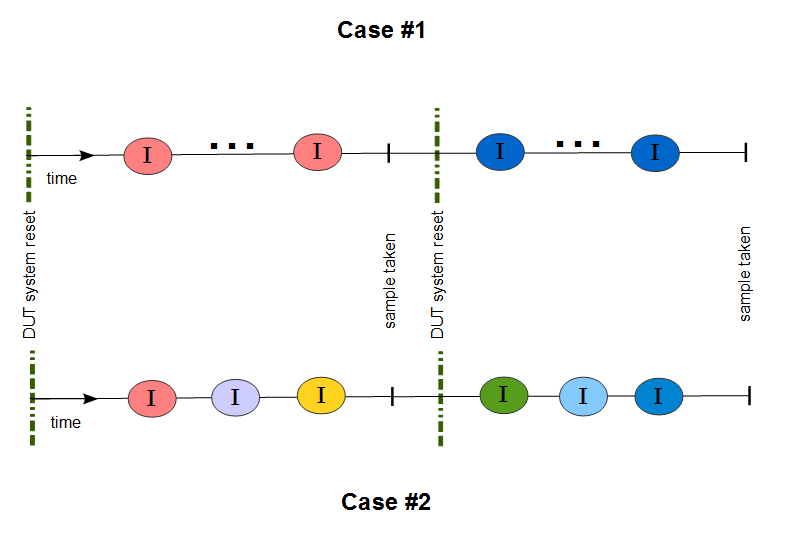
\includegraphics[width=0.85\linewidth]{../technical_diags/f8_changes_in_fault_sets_between_within_resets}
	\caption{Two ways multiple faults can change within and between system resets. Faults of different colors denote faults with different fault parameters. The group of faults between DUT system resets is a “fault set”.}
	\label{fig:two_ways_sets}
\end{figure}

Faults are generated on the fly meaning that whenever a fault injection occurs, fault characteristics values are generated. The fault injection system does not keep a list of faults, instead it keeps track of initial values, how characteristics change, and acceptable values for each characteristic. Faults can be generated non-randomly or randomly.

Non-random faults are generated by applying an arithmetic operation to a fault characteristic that yields values within a certain range. So every time a new fault is generated, the appropriate fault characteristic is “updated” by applying an arithmetic operation on that fault characteristic. Hardware checks that the resulting value is within bounds of a specified minimum and maximum.

Randomly generated characteristics can have four different probability distributions. The distributions available are unimodal Gaussian, bimodal Gaussian, uniform uniform, and uniform average. 

Remember that multiple fault characteristics can change. How does each fault characteristic change in relation to other fault characteristics? There are two ways to describe how multiple fault characteristics can change relative to each other; parallel and tree-like. In parallel change, multiple fault characteristic change at the same time without being affected by other changing fault parameters. In tree-like change, fault characteristics change in a parallel fashion while another fault characteristic stays constant, but that "constant" fault characteristic can change after a certain number of fault generation requests. 

For example, let’s say a fault can be characterized by its location and its type, and we are changing both characteristics. In parallel change, every time a new fault is generated (either in case 1 or case 2 of Figure \ref{fig:two_ways_sets}) both the location and type are updated. In tree-like change, every time a new fault is generated, one of the two fault characteristics will be updated. The other parameter would only be updated after a certain number of updates to the changing parameter. So for a given value for one of the fault characteristic, there will be groups of faults sharing one fault parameter value, but having different values for the other parameters. Figure \ref{fig:faultparameterupdating} demonstrates the difference between parallel change and tree-like change. 

\begin{figure}[h]
	\centering
	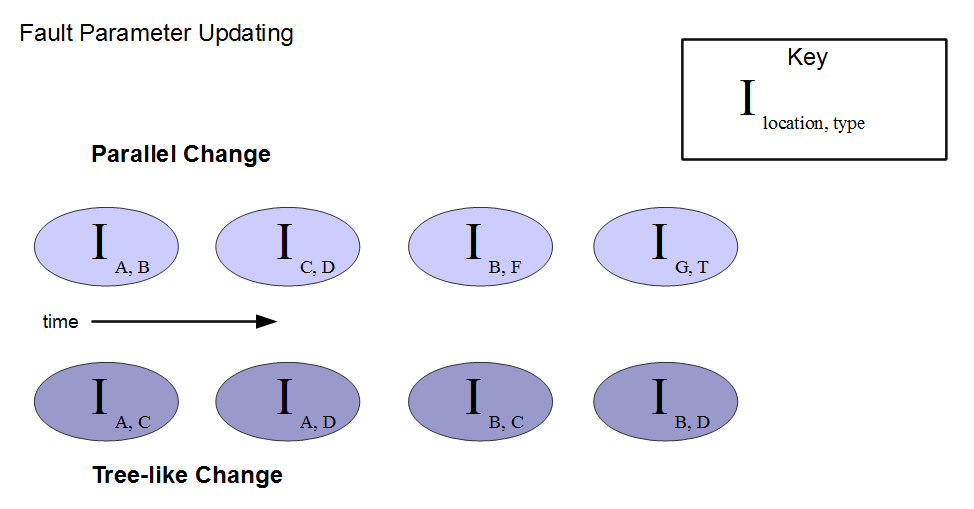
\includegraphics[width=0.7\linewidth]{../technical_diags/f11_fault_parameter_updating}
	\caption{Fault Parameter Updating. Shows the difference between parallel and tree-like change.}
	\label{fig:faultparameterupdating}
\end{figure}

\subsubsection{Randomly Generated Injection Time}
\label{ss rand gen inj time}

Be careful when injection time is configured to be generated randomly. Since injection time can't be predicted in advance, not all faults within a set can be injected before sampling occurs. \textit{All} faults in a set must be injected \textit{before} sampling to avoid injection and sampling at the same time. The MISST system doesn't explicitly enforce each set to have the same number of fault injections before sampling so the MISST system should be configured with that in mind. 

Its recommended that if injection time is randomly generated, that sets be limited to only one fault. Make sure to set the appropriate bounds for this injection time so that it occurs before sampling time.

\subsection{Sampling Data}
\label{s sampling data}

When a sampling timer timeouts within the Control Unit, MISST samples data from the DUT and sends the data to a PC. The system can sample two locations per set if thats desired. MISST can also be configured to stop a fault campaign based on sampled data. See the Design Guide for more details.

\chapter{Adapter Setup}
\label{c adapter setup}

\section{Introduction}
In this chapter we explain how MISST system core communicates with a terminal device (usually a computer) and a DUT. The Adapter module communicates with the fault injection system using a specific protocol. However, how the adapter module communicates with the PC and the DUT is up to the adapter designer.

\section{Design Goals}
Separating the fault injection system's core implementation and external communication module allows the MISST system core to be independent of external communication needs and development board. The fault injection system won't be limited by the development board it's implemented on or available communication hardware. 

The adapter module is responsible for routing and controlling signals between the MISST core, a terminal device (usually a PC), and the DUT. A high level diagram of these connections is shown in Figure \ref{fig:adapter high level interconnect}.

\begin{figure} [h]
	\centering
	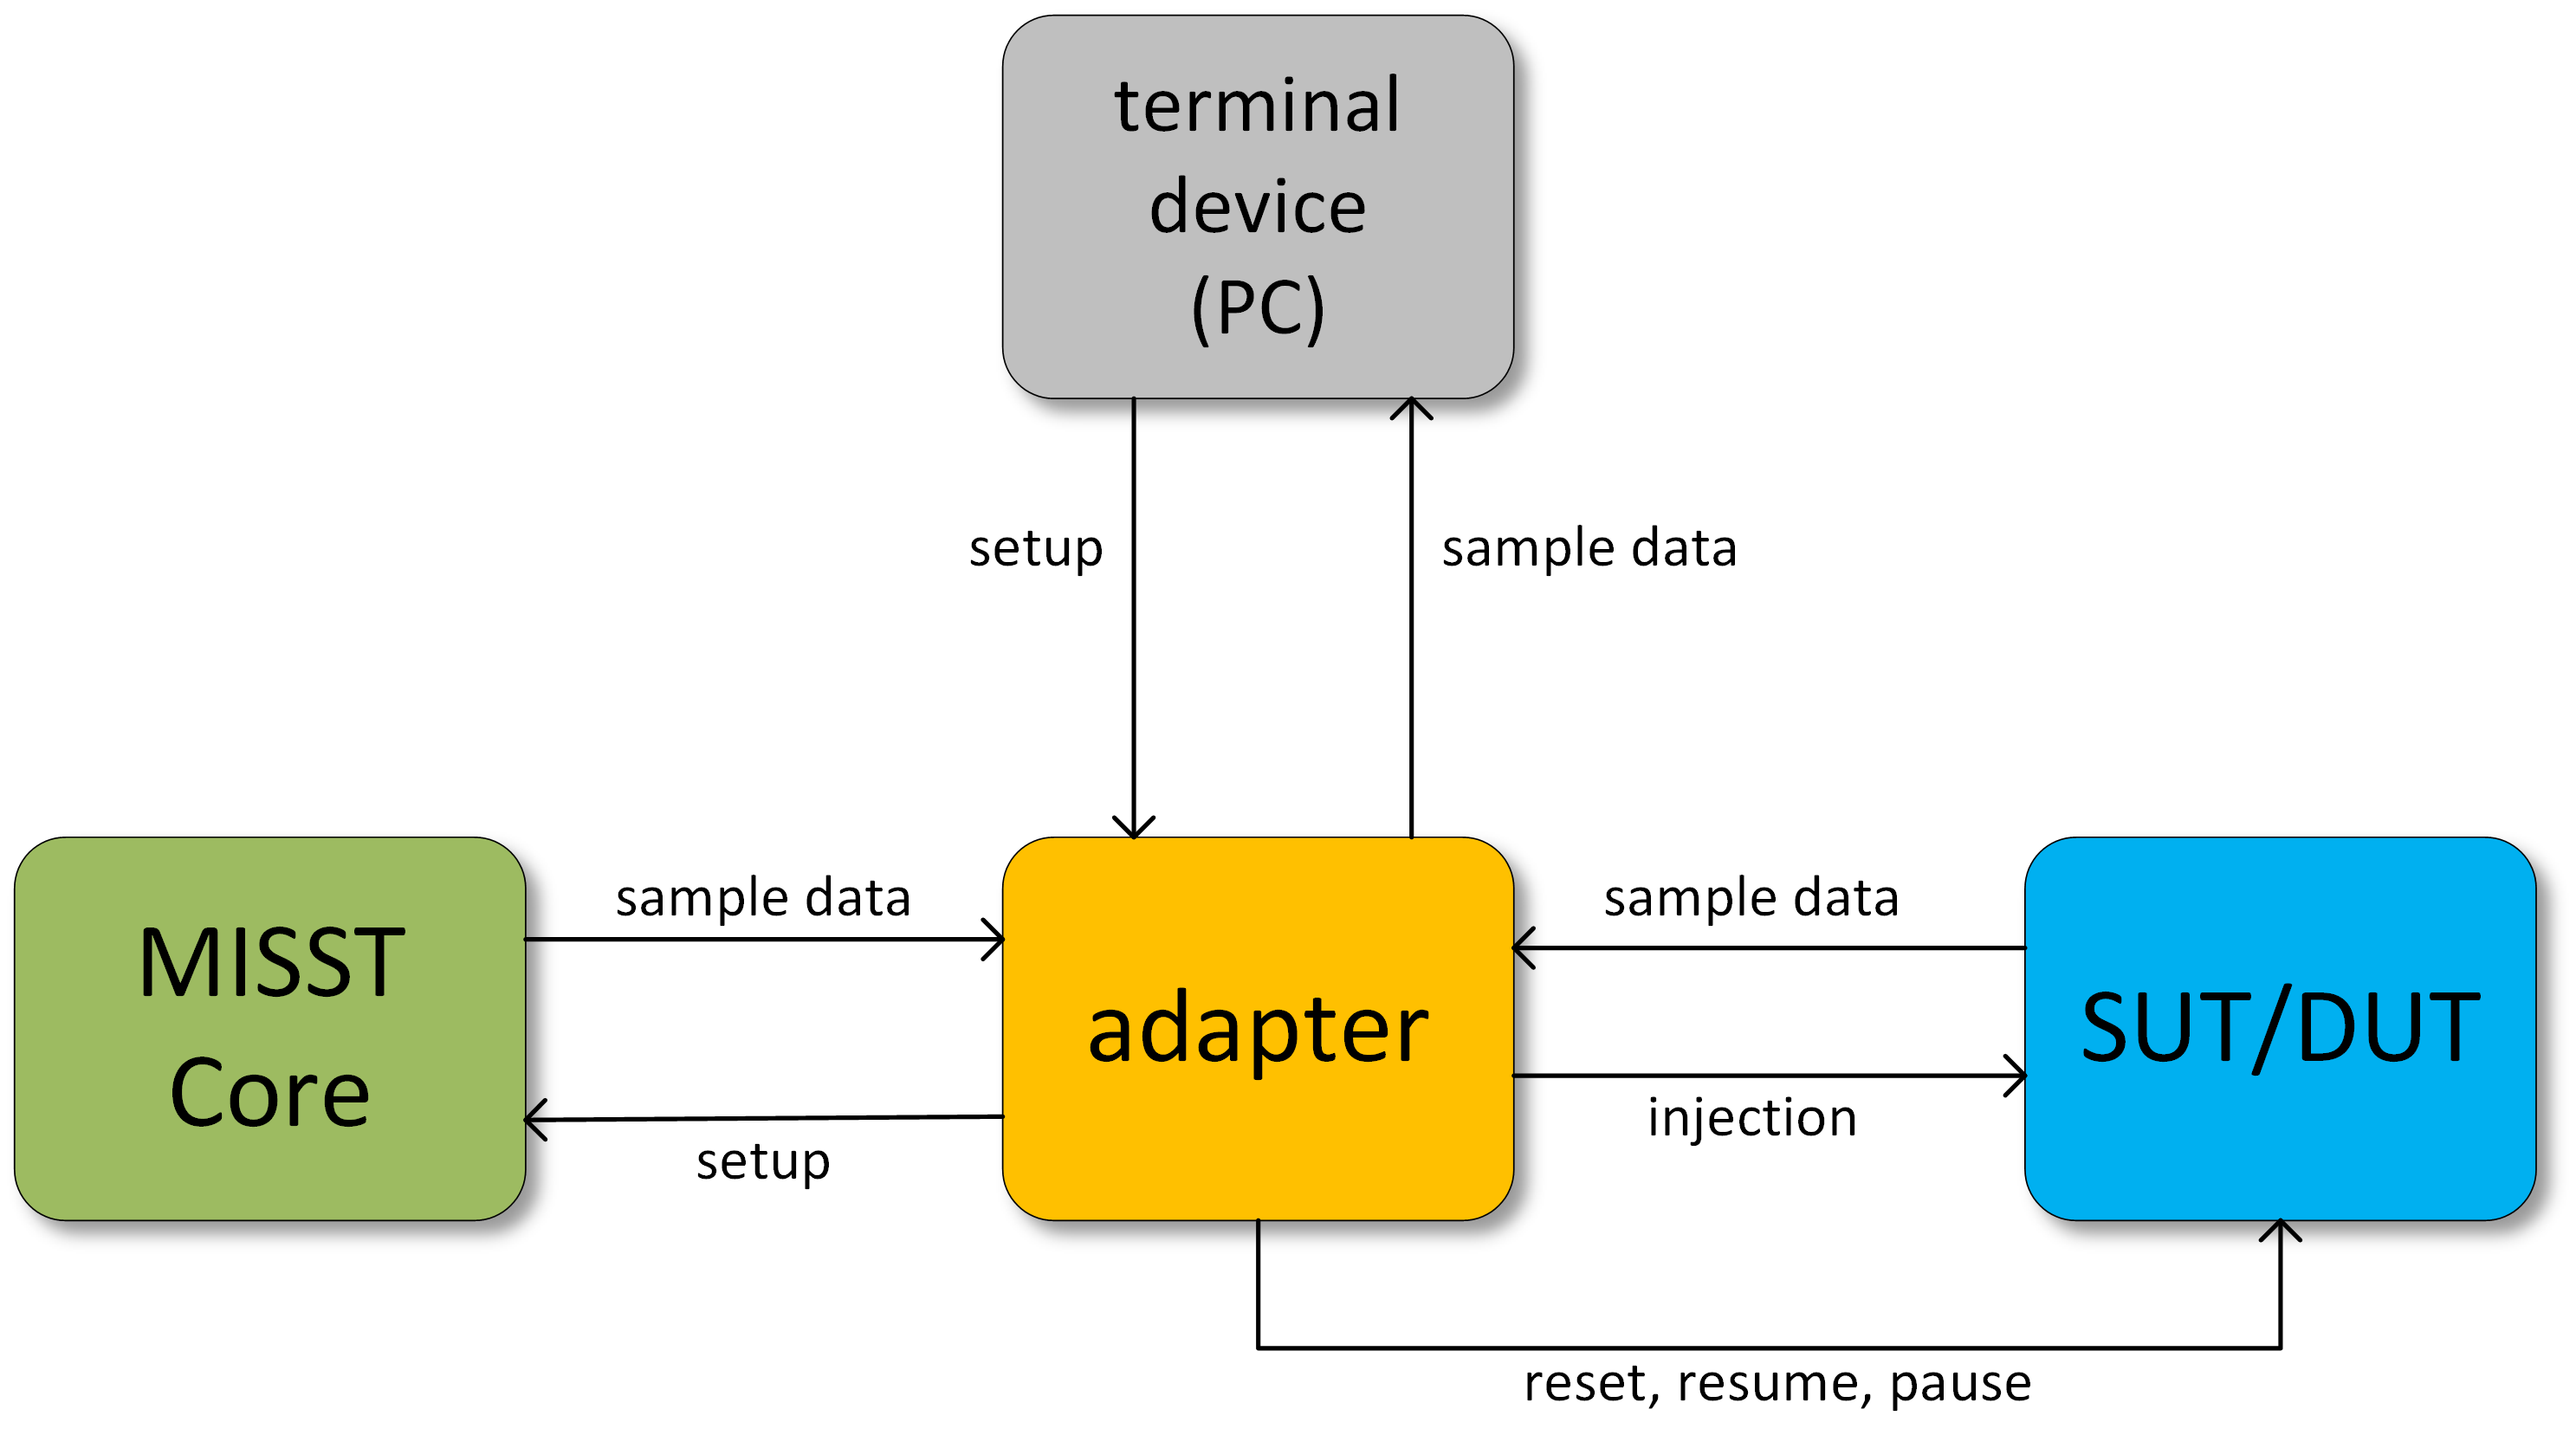
\includegraphics[width=0.7\linewidth]{../technical_diags/f16_core_adapter_pc_dut_high_level}
	\caption{High Level Adapter, MISST core, PC, and DUT Interconnect.}
	\label{fig:adapter high level interconnect}
\end{figure}


\section{Adapter-Core Communication Protocol}
\label{s adapter protocol}

The Adapter-Core Communication Protocol (ACCP) specifies how data is transfered between the adapter module and MISST core.  Table \ref{table:adapter required ports} lists and describes the required ports for the adapter. The only timing restriction is that the module sending data, be it the adapter module or MISST core, allow sufficient time for the receiver to process incoming data.

\begin{table}[h]
	\centering
	\caption{Required Adapter Ports}
	\begin{tabular}{|c|c|p{12cm}|}
		\hline 
		Port Name & I/O & Description \\ 
		\hline 
		data\_in & input & Data from MISST core. \\ 
		\hline 
		addr\_in & input & Destination address of incoming data. \\ 
		\hline 
		read\_in & input & Writes incoming data at incoming address on rising edge. \\ 
		\hline 
		campaign\_in & input & A high value signals system executing fault campaign. \\ 
		\hline 
		is\_sampling\_in & input & A high value indicates system during sampling process. \\ 
		\hline 
		is\_inj\_in & input & A high value indicates system during injection process. \\ 
		\hline
		samp\_inj\_in & input & A high value indicates that the value at the injection location is being read for corruption and injection. \\
		\hline 
		data\_out & output & Data to MISST core. \\ 
		\hline 
		addr\_out & output & Destination address of outgoing data to MISST. \\ 
		\hline 
		write\_out & output & Rising edge signals write enable for outgoing data at outgoing address to the Control Unit. \\ 
		\hline 
	\end{tabular} 
	\label{table:adapter required ports}
\end{table}

The user is free to add additional ports to the adapter as long as the required ports are included. Also note that the register sys\_status at address 0x0C (refer to Design Guide's \textbf{Memory Organization} section) is implemented in the adapter module. Hence the need for the sample\_in, inj\_in, and campaign\_in input ports. 

%---------------------------------------------------------------------
\part{Development Tips and Advice}

\section*{Introduction}
Here I will share helpful tips on working with Xilinx Vivado tools, VHDL, and Visio.

\section{Visio}

Visio is useful for creating block diagrams of system components. Visio allows users to create libraries of commonly used objects. I use this functionality to place multiple instances of a module. A useful Visio library is "Integrated Circuit Components". This library contains templates for block diagrams. Access it by following the steps outlined below:
\begin{enumerate}
	\item Open the "Shapes" left side-bar.
	\item Click on "More Shapes" and go to "Engineering", then "Electrical Engineering", and click on "Integrated Circuit Components".
	\item This library should now appear under "More Shapes" in the "Shapes" side-bar. You should be able to drag and drop objects from the side-bar to the canvas. 
\end{enumerate}

Once a design is ready, you can save the Visio design as a png file to include in documentation.
\begin{enumerate}
	\item Go to File-\textgreater Export-\textgreater Change File Type.
	\item Select "PNG Portable Network Graphics" under Graphic File Types. Click "Save As".
	\item Select directory to save and name file.
	\item Now you should see a window titled "PNG Output Options" as shown in Figure \ref{fig: png options window}. 
	\item Under "Resolution" select "Custom" and type 200 in the text fields with the 'X' between them (these text fields have 96 in Figure \ref{fig: png options window}).
	\item Under "Size" select Custom.
	\item Click ok and the png file should be in the directory you selected earlier.
\end{enumerate}

\begin{figure}[h]
	\centering
	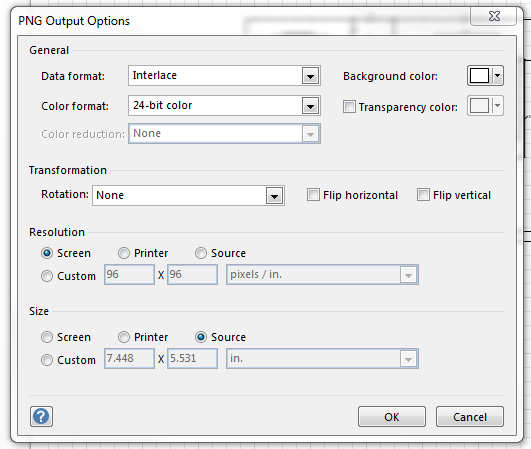
\includegraphics[width=0.7\linewidth]{../technical_diags/c14_png_options_window}
	\caption{PNG Output Options window.}
	\label{fig: png options window}
\end{figure}

\section{VHDL Tips}

When planning module implementation, keep the following VHDL rules in mind:
\begin{itemize}
	\item Signals can only be driven by one source. This means that a signal can be assigned values by combinatorial expressions or sequential expressions, \textit{but not both}. Furthermore, if driven sequentially, only one process at a time can assign values to a signal.
	\item A process only "runs" or, more accurately, assign values to driven signals when a signal in its sensitivity list changes. Use this to your advantage.  
	\item Conceptualize a process as mini-module with the sensitivity list as inputs and any signals the process drives as outputs. From the point of view of the synthesis tool, the sequential statements in a VHDL process outline an algorithm to map a series of inputs to a series of outputs.
	\item \textit{NEVER} use the std\_logic\_arith VHDL library, use numeric\_std instead. The std\_logic\_arith is not approved by the IEEE standardization body \cite{bad library site}.
	\item You can't read the values of entity output ports. Instead, use an internal signal that drives the output port combinatorially, and read the internal signal. 
\end{itemize}

Here is a list of VHDL style choices I followed throughout the project. Files created earlier in the project may not follow some of these style rules.
\begin{itemize}
	\item Internal signals have a "s\_" prefix. Early in the project, I used "t\_".
	\item Entity input ports have a "\_in" prefix.
	\item Entity output ports have a "\_out" prefix.
	\item Name processes to describe function.
	\item Include a reset port on moderately complex modules to initialize and reset registers and internal states.
\end{itemize}

\section{Implementation with Xilinx Vivado Tools}

I'm assuming that your previous experience with Vivado has been in a digital design course so this section won't be an introduction to Vivado. Instead, I'll share tips that could be helpful in the design and testing process.

Whenever Xilinx tools ask for the board you are using, the PYNQ-Z1 part number is \textbf{xc7z020clg400-1}.

\subsection{Simulation}
Testing is an important aspect of development. Try to implement a module's features so that they are not dependent on others. Using this method, features can be tested separately throughout the development process. Before programming the FPGA, test modules with Vivado Simulation. This section will provide tips on making the testing process more efficient.

The source code for the testbench of moderately complex modules will be long, and so will the waveform diagrams. To know what test is running in the waveform window during simulation, create an enumerated type signal whose values correspond to tests in the testbench file. Use the \textit{type} keyword to create an enumeration type. An example architecture section of a testbench is shown below. During the simulation, make sure to add the signal of the enumerated type to the waveform window if not already included. Adding this signal will help you visualize the start and end times of tests.

\begin{verbatim}
architecture behavior of testbench is
    type TEST_NAME is (TEST_1, TEST_2, TEST_3);
    ...
	signal test_name: TEST_NAME := TEST_1;
	...
begin
    ...
    stim_proc: process
    	...
    	test_name <= TEST_2;
    	...
    	test_name <= TEST_3;
    	...
    	wait;
    end process;
end;
\end{verbatim}

Be aware that in the waveform window you can change the colors of each waveform. You can also create dividers by right clicking in the name column of signal names and selecting the "New Divider" option. Figure \ref{fig:wave form window example} shows an example of a waveform window.

\begin{figure}[h]
	\centering
	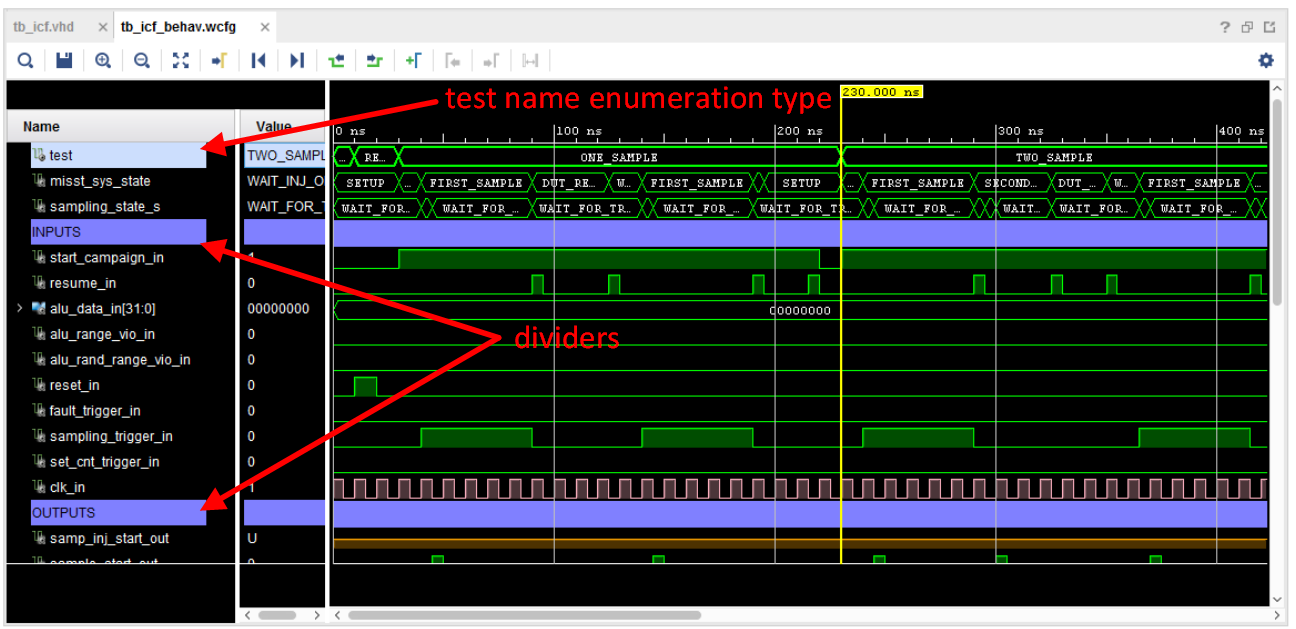
\includegraphics[width=1.0\linewidth]{../technical_diags/f23_waveform_window_example}
	\caption{Waveform Window Example.}
	\label{fig:wave form window example}
\end{figure}

\subsection{Creating AXI Peripheral}
\label{ss creating axi ip}
You must create an AXI slave peripheral IP to use in the overall system block design in section \ref{ss configurating pynq processor}. I refer you to chapter 3 of \cite{creating ip}. Start at the beginning of the chapter and when you arrive to step 3 on page 23, continue the steps for "Create a new AXI4 peripheral". For step 5, do not include interrupts. For step 7, select "Edit IP" to add Adapter-Core Communication Protocol logic to the AXI slave (see section \ref{s adapter protocol} for protocol requirements).  

In the template generated by Vivado, do not heavily modify the AXI protocol logic unless you know what you are doing. To avoid confusion between user code and AXI code, implement your code where comments suggest you do so. For example, you should add any combinatorial logic between the comments below.
\begin{verbatim}
-- Add user logic here

-- User logic ends
\end{verbatim}
You should add ports between the comments below.
\begin{verbatim}
-- Users to add ports here

-- User ports ends
\end{verbatim}
The point is to avoid confusing the template code and your code.

\subsection{Configuring the PYNQ Processor}
\label{ss configurating pynq processor}

This section will explain how to integrate the PYNQ processor, the AXI slave interface, and any DUT interfaces to create the bit-stream necessary to program the PYNQ board.

The entire MISST setup will be done in a block design. As example block design is shown in Figure \ref{fig:adapter block design example}.

\begin{figure}[h]
	\centering
	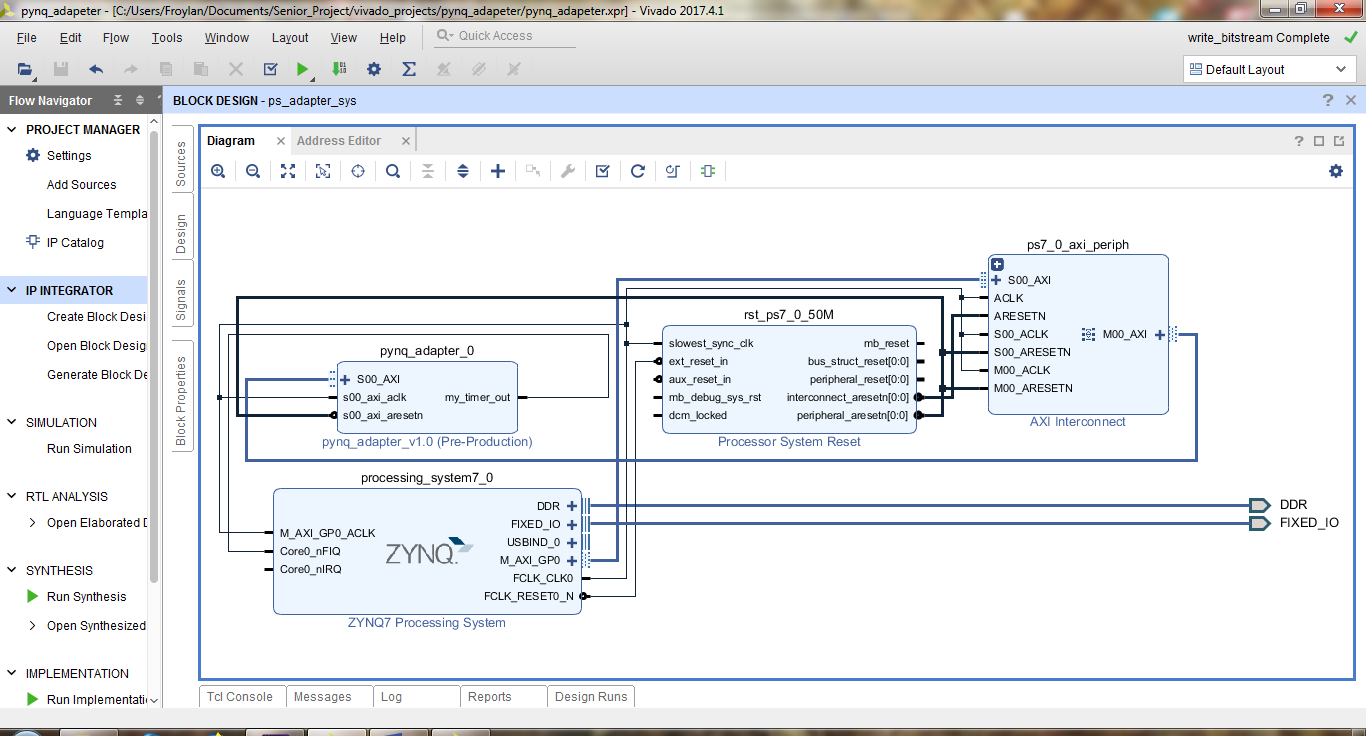
\includegraphics[width=0.7\linewidth]{../technical_diags/c16_adapter_block_design_example}
	\caption{Example Block Design with PYNQ Processor.}
	\label{fig:adapter block design example}
\end{figure}

The block pynq\_adapter\_0 is an AXI slave of the processor represented by the processing\_system9\_0 block. The name of each block as listed in the IP library is shown below each block. Also note that the input ports core0\_nFIQ and core0\_nIRQ are interrupt inputs for the PYNQ processor.

Chapter 2 of reference \cite{ug zynq embedded design} details how to create an embedded design with the processor from project creation to processor programming. Watch out for the following when carrying out instructions in \cite{ug zynq embedded design}:
\begin{itemize}
	\item On page 15, the "Board" property of "Default Part" should be set to xc7z020clg400-1 as previously mentioned.
	\item Step 2 of page 17 is \textit{very} important. The preset template is a .tcl script that tells Vivado what resources are available on the ZYNQ chip on the PYNQ board. The file is called pynq\_revC.tcl and is available at \cite{pynq docs and support files}.
\end{itemize}

To include logic fabric triggered interrupts on the processor, go to the "Interrupts" page on the "Re-customize IP" window for the PYNQ processor and click on "Fabric Interrupts", click "PL-PS Interrupt Ports", and select "IRQ\_F2P[15:0]".

\subsection{Programming PYNQ Processor with SDK}

At this point, you should have imported the bit-stream of the design block to SDK, and opened a simple 'Hello World' project template.

The SDK will create a header file that provides read and write functions to an AXI slave peripheral. If we have an AXI slave called IO\_Bridge, then the write and read functions will be implemented in header file io\_bridge.h. The read and write functions are shown below.
\begin{verbatim}
	#include "io_bridge.h"
	
	// write 0x01 to AXI slave 0 at register 0
    IO_BRIDGE_mWriteReg(XPAR_IO_BRIDGE_0_S00_AXI_BASEADDR, IO_BRIDGE_S00_AXI_SLV_REG0_OFFSET, 0x00000001);
	
	// read register 3 from AXI slave 0 and save in unsigned integer variable axi_data
	axi_data = IO_BRIDGE_mReadReg(XPAR_IO_BRIDGE_0_S00_AXI_BASEADDR, IO_BRIDGE_S00_AXI_SLV_REG3_OFFSET);
\end{verbatim}

To print data to a PC, use the following functions:
\begin{verbatim}
	#include "xil_printf.h"
	
	// simple print to terminal
    print("Welcome!\r\n");

	// print variable value to terminal
	xil_printf("result: %0x\r\n", axi_data);
\end{verbatim}

View terminal output by opening a "Terminal" view in the SDK. To open a "Terminal" view in the SDK, follow the instructions on page 27 of \cite{ug zynq embedded design}.

%---------------------------------------------------------------------
\part{Project Status}

\section*{Quick Note}
As of June 16, 2018, the MISST system core is partly implemented. The following sections describe which features are implemented, and which are not. The source code for each module also list needed features. 

\section{The ALU}
The ALU is functionally complete, however, its random functions could be expanded. As of now, if the ALU was used in a complete MISST system, the system would function. The following additions will broaden the types of errors the ALU can produce.
\begin{itemize}
	\item Expand random number generation from 16-bit output to 32-bit output. The module used for random number generation, noise\_gen, uses a linear feedback shift register implementation to produce random value with four probability distributions. Due to noise\_gen's implementation, expansion to 32-bit output will be challenging if not impossible.
	\item Add functions that mimic single event upsets (a single bit is inverted in a group of data). The current single bit inversion operation only inverts a single bit within the least significant byte of operand A. Maybe expand this to within four bytes, or a byte other than the least significant byte.
	\item Add random number generator with Poisson distribution.
	\item Include random number generator with distribution specific parameters like average, variance, etc. Such a random number generator would produce random variables with a selected probability distribution and associated parameters.
\end{itemize}

\section{Fault Parameters}
The Fault Parameters module is complete. I don't see why Fault Parameters would have to be expanded, unless future developers deem it necessary to add another fault parameter.

\section{The Control Unit}
The Control Unit consists of three modules and three cycle counter modules. The three main modules are the register controller, the memory interconnect, and the injection campaign FSM (ICF). In summary:
\begin{itemize}
	\item The register controller processes data between MISST system core and Adapter module.
	\item The memory interconnect contains MISST system registers and forwards data to the Fault Parameter module.
	\item ICF is the brains of the MISST system coordinating signals necessary for injection and sampling operations to be carried out properly.
\end{itemize} 

The register controller and memory interconnect are complete. If any more registers are added to the MISST system, then memory interconnect would have to be updated accordingly.

The ICF is not complete. The injection process and shutdown check have not been implemented. The sampling process, however, has been implemented. The shutdown check refers to the ICF stopping the fault campaign when the number of sets has reached the maximum value. The steps in an injection process are outlined in the \textbf{Task Flow} section of the Design Guide.

\section{Adapter Module}
There is currently no Adapter module implementation, but how it will function, the ports needed, and development steps are known. The plan is outlined below.
\begin{enumerate}
	\item Create an AXI-Lite peripheral IP core in Vivado. Vivado automatically generates a template that includes AXI-Lite protocol logic. All the user needs to do is add their logic. Section \ref{ss creating axi ip} goes over how to accomplish this.
	\item Test AXI slave. I don't know how to test an AXI interface so I'd recommend testing the logic you implemented by making sure the AXI registers are written and read from properly. \textit{Do not heavily modify the AXI-Lite procotol logic.}. If you do, you might need to test the AXI interface itself which I'm not sure how to do.
	\item Package AXI-slave IP.
	\item Open a new Vivado project and create a block design. In this block design connect the PYNQ's hard processor, the PYNQ processor system, to the AXI slave (which should be connected to MISST), and the DUT (along with whatever interfaces needed). The ultimate goal of this step is to generate the bit-steam of the block design. See section \ref{ss configurating pynq processor} for instructions.
	\item  Export the bit-stream to the SDK (Software Development Kit) to program the hard processor. Refer to \textbf{Role of Cortex Processor} section of Design Guide for processor behavior.
	\item Program the FPGA, and then program the hard processor. 
	\item Setup MISST registers through the PC, and start fault campaign when ready.
\end{enumerate}

\section{Module Verification}

I consider a feature implemented if it has been simulated and verified to function as planned. All previously mentioned features have been tested and verified to work. However, these tests are unit tests. I haven't tested if the submodules of the Control Unit function \textit{together}. So when I say that the sampling process has been implemented for the ICF, I mean that the ICF can carry out its role in the sampling process i.e. turn on and off the ICF ports in the correct sequence to read data from the DUT. 

\section{Suggested Target DUT}

When the MISST system core and Adapter module are implemented, I suggest the following target systems.
\begin{itemize}
	\item LEON3: An open source 32-bit microprocessor core. The LEON3 is well documented and configurable, and its VHDL source code is available online. Source code, dependencies, and instructions on implmenting the LEON3 processor can be found at \cite{leon3}.
	\item MIAOW: Acronym for Many-core Integrated Accelerator Of Waterdeep/Wisconsin, is the only open source GPU freely available online. Note that the MIAOW requires roughly four times as many look-up tables as the ZYNQ FPGA has available. So to test on MIAOW must be implemented on a larger FPGA.Information about MIAOW can be found at \cite{meow gpu}.
\end{itemize}

\begin{thebibliography}{5}
	\bibitem{bad library site} 'Why the library "numeric\_std" is preferred over "std\_logic\_arith" and others', 2010. [Online]. Available: http://vhdlguru.blogspot.com/2010/03/why-library-numericstd-is-preferred.html. [Accessed: 5 April 2018].
	
	\bibitem{pynq board manual}PYNQ-Z1 Board Reference Manual. (2018). [ebook] Pullman. Available at: https://reference.digilentinc.com/\_media/reference/programmable-logic/pynq-z1/pynq-rm.pdf [Accessed: 24 Feb. 2018].
	
	\bibitem{ug zynq embedded design}Zynq-7000 All Programmable SoC: Embedded Design Tutorial. (2015). [ebook]. Available at: https://www.xilinx.com/support/documentation/sw\_manuals/xilinx2015\_1/ug1165-zynq-embedded-design-tutorial.pdf [Accessed: 6 May 2018].
	
	\bibitem{pynq docs and support files} PYNQ-Z1. [Online]. Available: https://reference.digilentinc.com/reference/programmable-logic/pynq-z1/start [Accessed: 6 May 2018].
	
	\bibitem{creating ip} Vivado Design Suite User Guide Creating and Packaging Custom IP. (2015). [ebook]. Available at: https://www.xilinx.com/support/documentation/sw\_manuals/xilinx2017\_2/ug1118-vivado-creating-packaging-custom-ip.pdf [Accessed: April 8, 2018].
	
	\bibitem{leon3} 'LEON3 Processor', [Online]. Available: https://www.gaisler.com/index.php/products/processors/leon3
	
	\bibitem{meow gpu} 'MIAOW GPU', [Online]. Available: http://miaowgpu.org/
	
\end{thebibliography}


\end{document}          
